\documentclass[]{article}
\usepackage[T1]{fontenc}
\usepackage[utf8]{inputenc}
%\usepackage[icelandic]{babel}
\usepackage{caption}
\usepackage{circuitikz}
\usepackage{grffile} 
\usepackage[margin=0.4in]{geometry}

% grffile er pakki sem leifir manni að nota "" til þess að forðast að nota
% nafnið á myndinni með.
\usepackage{graphicx}
% \graphicspath{{images/}} Sýnir undir möppu þar sem myndirnar eru

\usepackage{hyperref}
%fyrirlinka - \url{www.....}
\begin{document}


\title{Bókhald}
\author{Pétur}
\maketitle

\section*{E3.3}

Carillo Painting collected £108,000 from customers in 2020. Of the amount collected, £25,000 was for services performed in 2019. In addition, Carillo performed services worth £36,000 in 2020, which will not be collected until 2021.\\ 
Carillo Painting also paid £72,000 for expenses in 2020. Of the amount paid, £30,000 was for expenses incurred on account in 2019. In addition, Carillo incurred £42,000 of expenses in 2020, which will not be paid until 2021. 
\subsection*{a) Compute 2020 cash-basis(Greðslugrunnur) net income.}
£133,000=£108,000+£25,000
\subsection*{b) Compute 2020 accrual-basis(Rekstragrunnur) net income}
£108,000

\section*{E3.4}
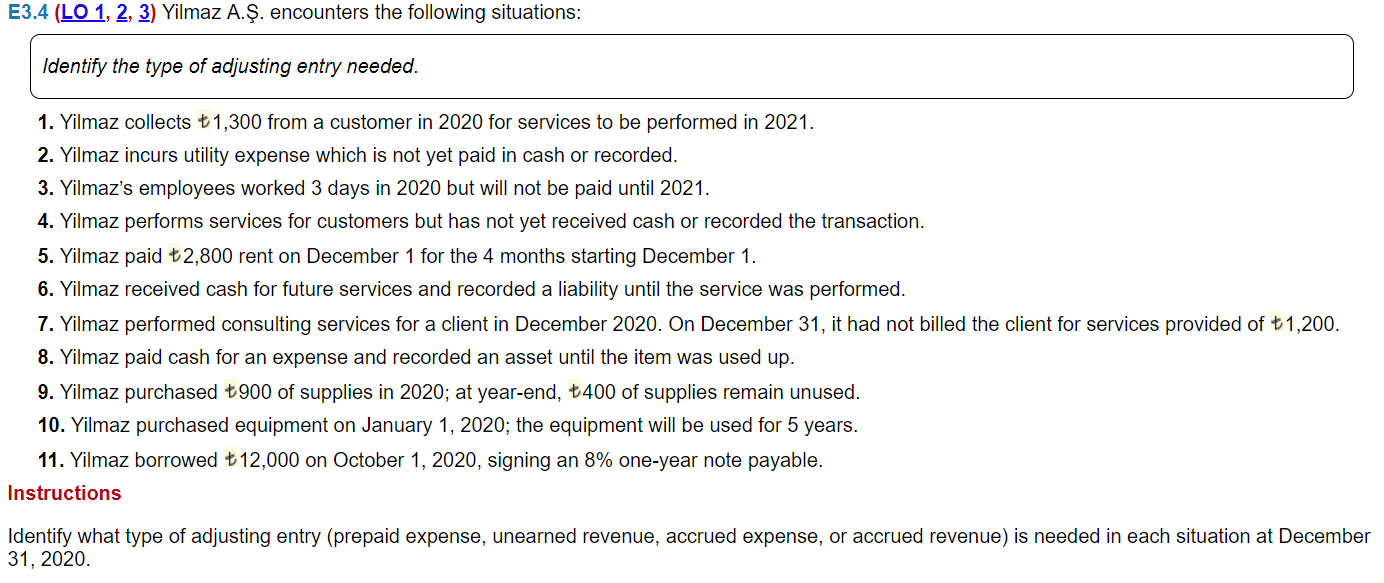
\includegraphics[scale=0.7]{E34}

\section*{E3.5}
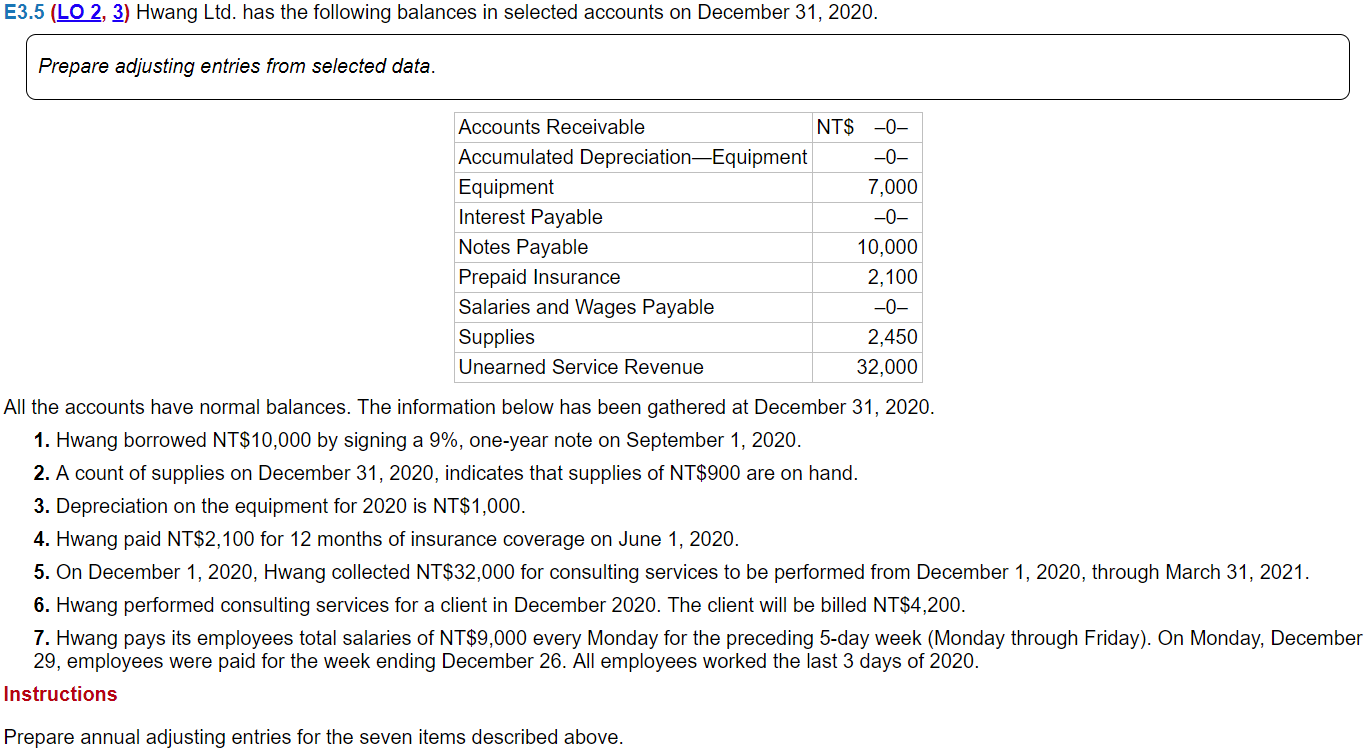
\includegraphics[scale=0.7]{E35}

\section*{E3.17}
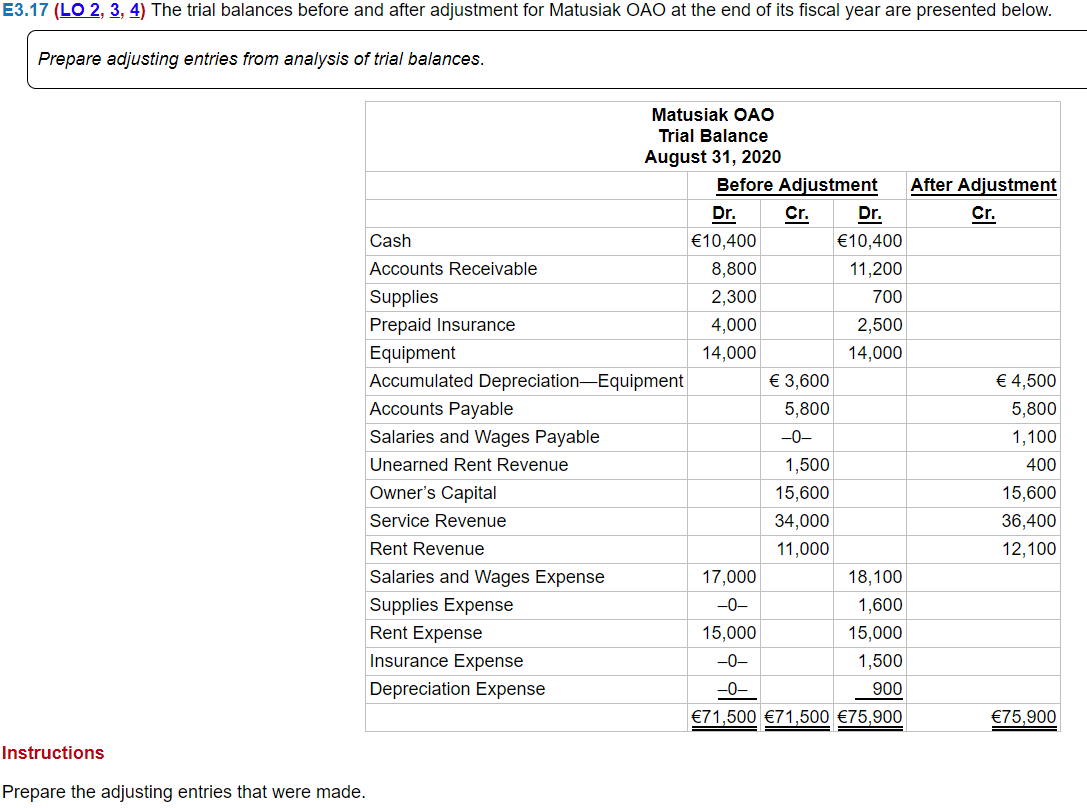
\includegraphics[scale=0.85]{E317}
\end{document}
